\documentclass[12pt]{article}
\usepackage[T1]{fontenc}
\usepackage[ngerman]{babel} % german as language
\usepackage{csquotes}
\usepackage[onehalfspacing]{setspace} % 1.5 Zeilenabstand
\usepackage{parskip} % for paragraph line skip
\usepackage{fancyhdr} % for headers
\fancyhf{}
\fancyhead[C]{\nouppercase{\firstmark}}
\renewcommand{\headrulewidth}{0pt} % change line under header
\renewcommand{\footrulewidth}{0pt}
\pagestyle{fancy}
\setlength{\headheight}{15.04742pt}
\fancypagestyle{maintext}{ % pagestyle for main text for page numbers
    \fancyhf{}
    \fancyhead[C]{\nouppercase{\firstmark}}
    \fancyfoot[C]{\thepage}
    \renewcommand{\headrulewidth}{0pt}
    \renewcommand{\footrulewidth}{0pt}
}
% Update \sectionmark to show first section in header
\renewcommand{\sectionmark}[1]{%
    \markboth{\thesection\ #1}{}
}
\renewcommand{\subsectionmark}[1]{}

% for tables/figures
\usepackage{graphicx}
\usepackage{caption}
\usepackage{array}
\graphicspath{ {figures/} } % set path to figures
\renewcommand{\listfigurename}{Abbildungsverzeichnis}
\renewcommand{\listtablename}{Tabellenverzeichnis}

% Appendix
\usepackage[toc,page]{appendix}
\renewcommand\appendixname{Anhang} % Change name to German
\renewcommand\appendixpagename{Anhang}
\renewcommand\appendixtocname{Anhang}


% \usepackage{sectsty} -> falls section font size 14 haben muss
% \sectionfont{\large\bfseries}

% use geometry for page layout
\usepackage[a4paper, left=2.5cm, right=2.5cm, top=2.5cm, bottom=2cm]{geometry}

% Citation: BibLaTeX als author-year style, benötigt xelatex->biber->xelatex(2x) als recipe!
\usepackage[
backend=biber,
style=authoryear]{biblatex}
\addbibresource{refs.bib}

% Start des Dokuments
\begin{document}

% Add centered Title page
\begin{titlepage}
    \begin{center}
        \vspace*{0.5cm}
            
        \LARGE
        \textbf{HHH \enquote{fiktive Waren} im 21. Jahrhundert}
            
        \vspace{0.2cm}
        \Large
        Das hier ist noch ein weiterer Test\\

            
        \vspace{2cm}
            
        \textbf{Lukas Schaffrath}\\
        Matrikelnummer: 411793\\
        Lehramt Technik/Englisch\\
        Master für Gymnasien und Gesamtschulen
            
        \vspace{2cm}
            
        Ringseminar Transformationssoziologie\\
        Dozent: Tim Franke
            
        \vspace{2cm}
            
            
        \Large
        Institut für Soziologie\\
        Lehrstuhl für Technik- und Organisationssoziologie\\
        RWTH Aachen University\\
        Wintersemester\\
        19. November 2024
            
    \end{center}
\end{titlepage}

% % Add table of contents with emtpy page number
% \addtocontents{toc}{\protect\thispagestyle{empty}}
% \tableofcontents

% % List of figures and tables
% \newpage
% \thispagestyle{empty}
% \listoffigures
% \vspace{0.5cm}
% \listoftables


% New page, page count to 1
\newpage
\setcounter{page}{1}
\pagestyle{maintext}

% Add Main Text
\section{Einleitung}
In dieser Hausarbeit wird eine beispielhafte 


\section{Grundlagen}
Im Folgenden werden die Grundlagen, auf denen die theoretische Ausarbeitung der Unterrichtsreihe beruht, vorgestellt, um ein bestmögliches Verständnis für die Auswahl der didaktischen Praktiken zu ermöglichen. Für die gestaltung einer Unterrichtsreihe, die besonders inklusives Lernen innerhalb einer heterogenen Schüler-Gruppe fokussiert, muss der Begriff der Heterogenität und des inklusiven Lernens definiert werden, was im ersten Unterkapitel versucht wird. Des Weiteren werden die zwei Förderschwerpunkte, die in der vorgestellten Lerngruppe vorkommen, spezifiziert und Hinweise auf den Umgang mit 


\vspace{0.8cm}

% \begin{center}
%     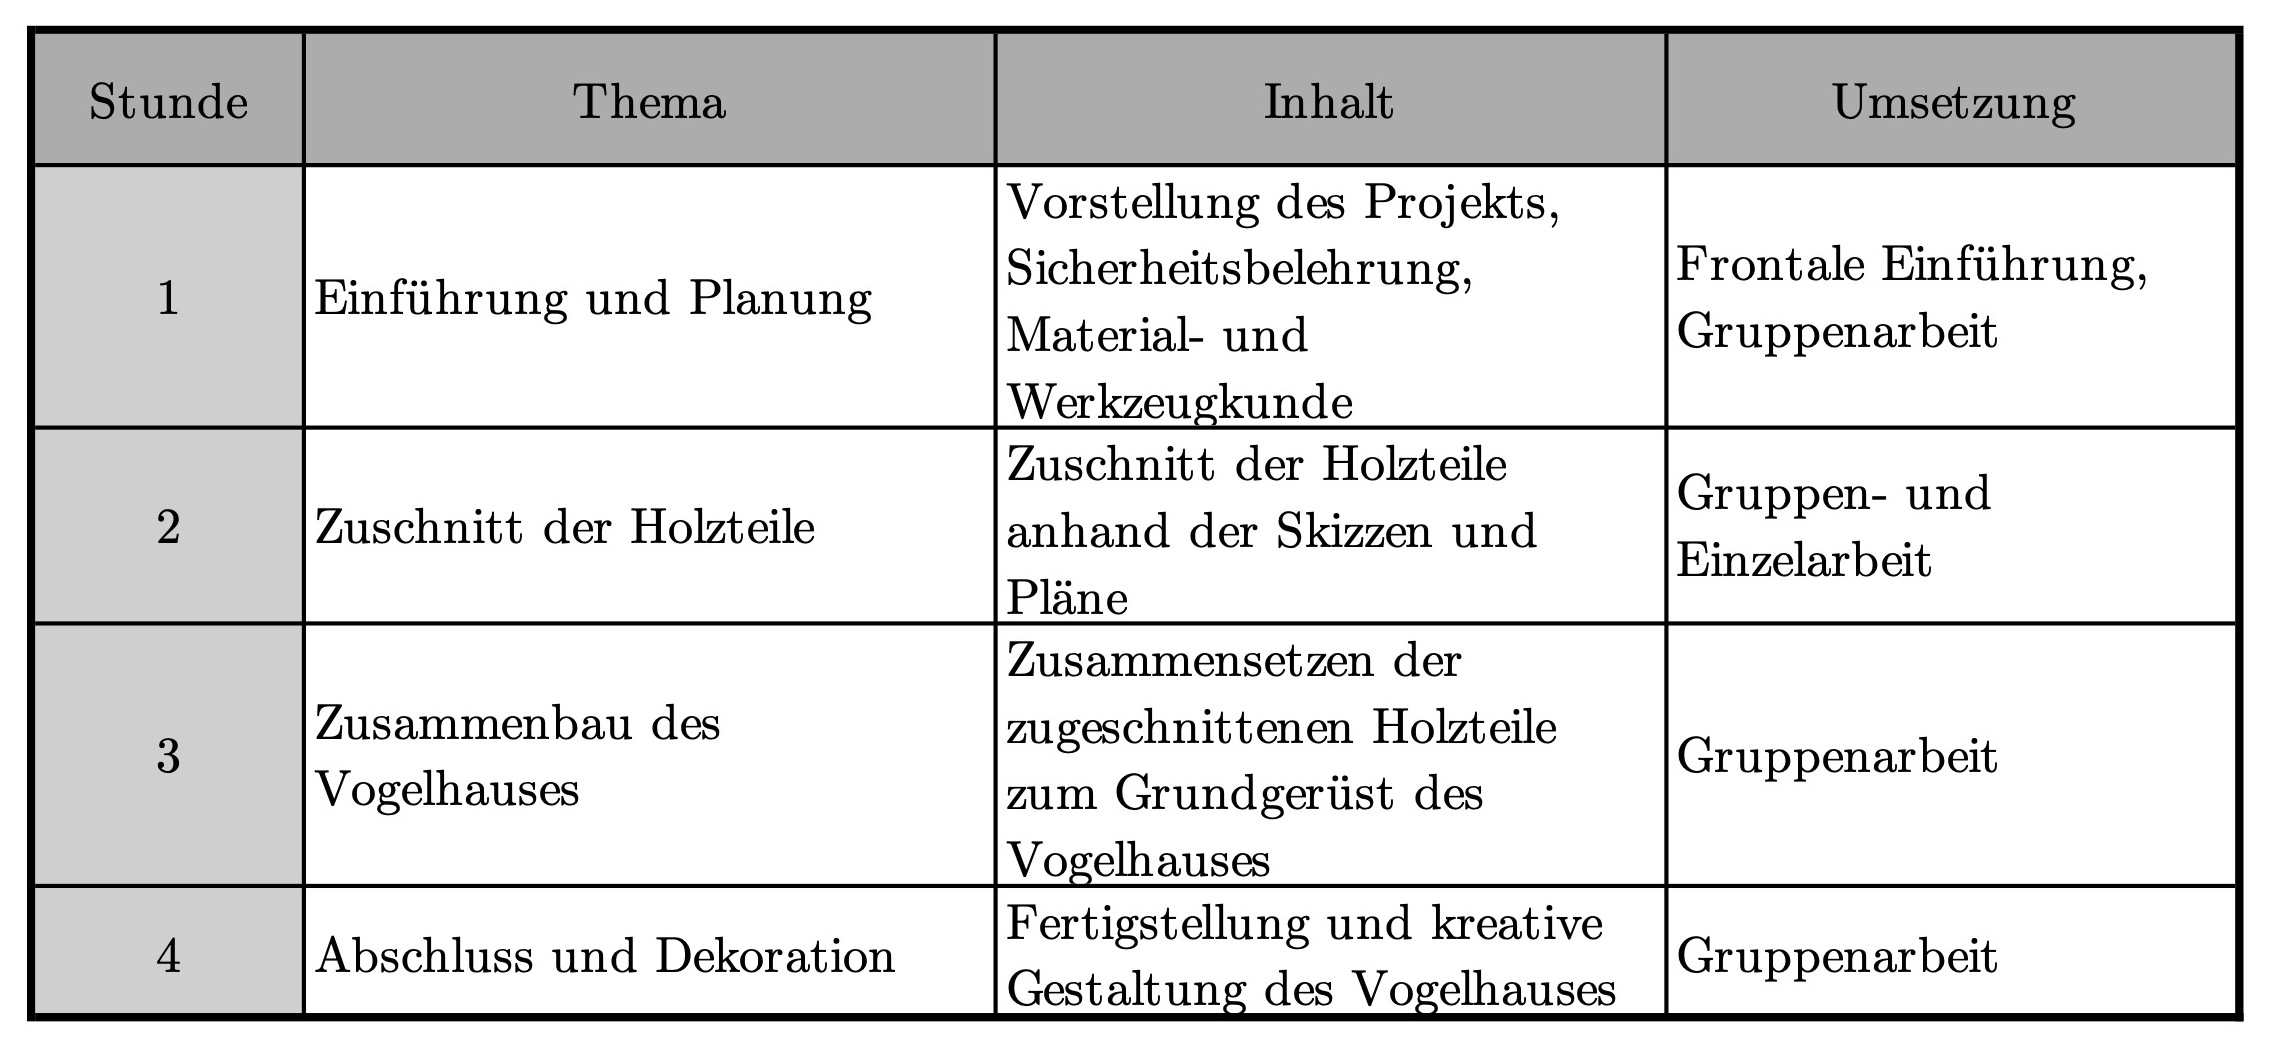
\includegraphics[height=6cm, angle=0, keepaspectratio]{static/Unterrichtsverlauf_Tabelle.jpg}
%     \captionof{table}{Tabellarischer Verlaufsplan der Unterrichtsreihe}
% \end{center}

% Die Schülerinnen und Schüler...
% \begin{itemize}
%     \item können die Bauteile eines Vogelhauses benennen und verstehen deren Zusammenhang.
%     \item können einen personalisierten Bauplan für ein Vogelhaus erstellen, indem sie ihre bisherigen Erfahrungen kreativ zum Ausdruck bringen.
%     \item benennen und begründen ihre Überlegungen sachgerecht.
% \end{itemize}


% print bibliography with heading in table of contents
\newpage
\printbibliography[heading=bibintoc]
\pagestyle{empty}

% Starte Anhang
\newpage
\begin{appendices}

    % Sektionen
    % \section{Tabellarischer Verlaufsplan zur ersten Unterrichtsstunde}
    % \begin{center}
    %     \includegraphics[height=14cm, angle=90, keepaspectratio]{static/Unterrichtsstunde_1_Tabelle.pdf}
    %     \captionof{table}{Tabellarischer Verlaufsplan zur ersten Unterrichtsstunde}
    % \end{center}
    
    % \section{Tabellarischer Verlaufsplan zur zweiten Unterrichtsstunde}
    % \begin{center}
    %     \includegraphics[height=14cm, angle=90, keepaspectratio]{static/Unterrichtsstunde_2_Tabelle.pdf}
    %     \captionof{table}{Tabellarischer Verlaufsplan zur zweiten Unterrichtsstunde}
    % \end{center}

    % \section{Abbildung eines Beispielhaften Vogelhauses}
    % \begin{center}
    %     \vspace{1cm}
    %     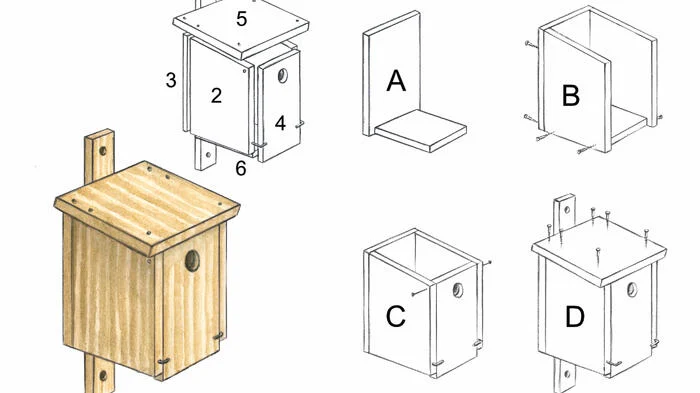
\includegraphics[width=10cm, keepaspectratio]{static/Beispiel-Vogelhaus.png}
    %     \captionof{figure}{Beispielhaftes Vogelhaus \parencite{noauthor_vogelhaus_nodate-1}}
    % \end{center}

    % \section{Folie zur Vorstellung des Bauplans}
    % \begin{center}
    %     \vspace{1cm}
    %     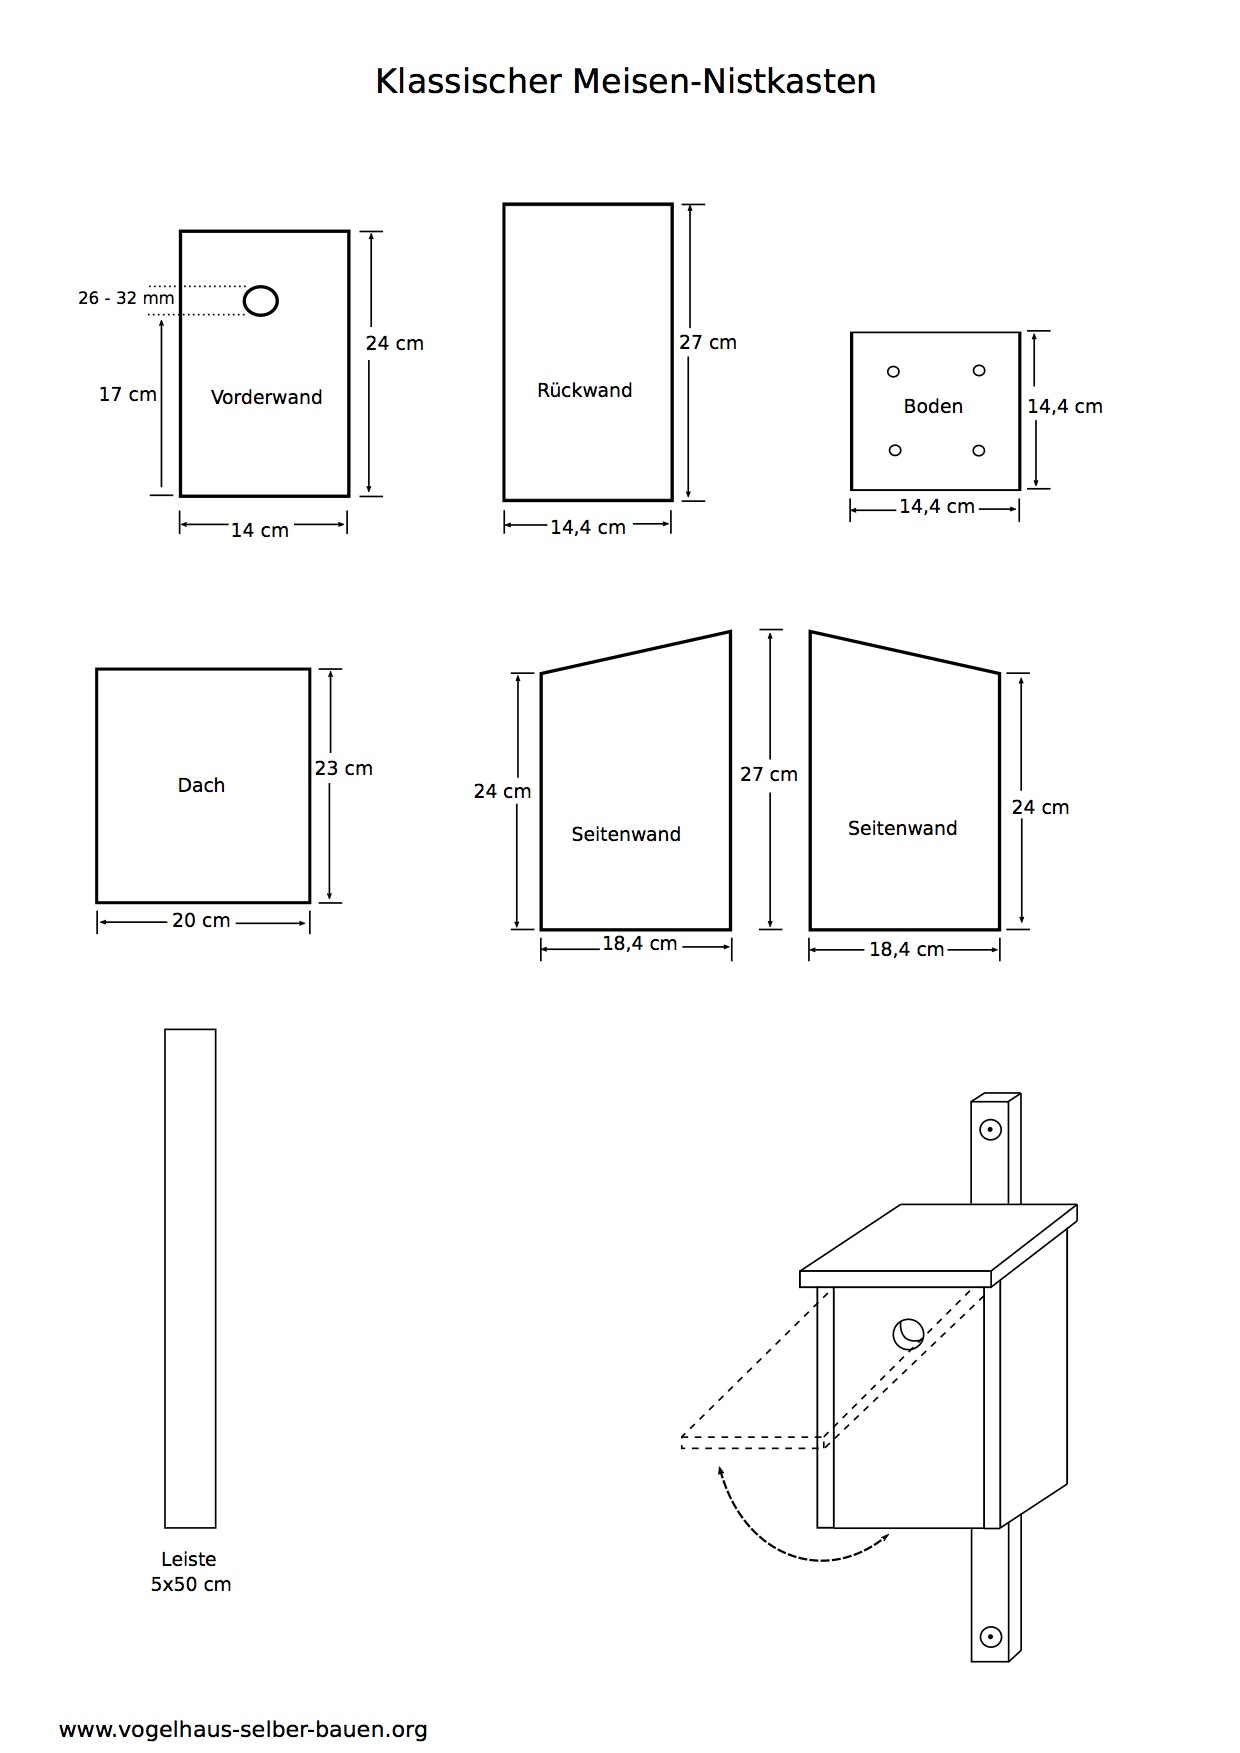
\includegraphics[width=10cm, keepaspectratio]{static/Bauplan-Vogelhaus.jpg}
    %     \captionof{figure}{Beispielhafter Bauplan \parencite{noauthor_vogelhaus_nodate}}
    % \end{center}

    % \section{Aufgabenblätter zur ersten Unterrichtsstunde}
    % \begin{center}
    %     \vspace{0cm}
    %     \includegraphics[height=21cm, keepaspectratio]{static/Aufgabenblatt1.pdf}
    %     \captionof{figure}{Aufgabenblatt 1 - Aufgabenstellung}
    %     \vspace{2cm}
    %     \includegraphics[height=21cm, keepaspectratio]{static/Aufgabenblatt2.pdf}
    %     \captionof{figure}{Aufgabenblatt 2 - Bauplan der Rückwand}
    %     \vspace{2cm}
    %     \includegraphics[height=21cm, keepaspectratio]{static/Aufgabenblatt3.pdf}
    %     \captionof{figure}{Aufgabenblatt 3 - Bauplan der Vorderwand}
    %     \vspace{2cm}
    %     \includegraphics[height=21cm, keepaspectratio]{static/Aufgabenblatt4.pdf}
    %     \captionof{figure}{Aufgabenblatt 4 - Bauplan der Seitenwand 1}
    %     \vspace{2cm}
    %     \includegraphics[height=21cm, keepaspectratio]{static/Aufgabenblatt5.pdf}
    %     \captionof{figure}{Aufgabenblatt 5 - Bauplan der Seitenwand 2}
    % \end{center}

    % \section{Sicherheitsbelehrung}
    % \begin{center}
    %     \vspace{2cm}
    %     \includegraphics[height=21cm, keepaspectratio]{static/Sicherheitsbelehrung.pdf}
    %     \captionof{figure}{Sicherheitsbelehrung}
    % \end{center}

    \section{Eidesstattliche Versicherung}
    \begin{center}
        \vspace{2cm}
        \includegraphics[height=21cm, keepaspectratio]{static/Eidesstattliche-Versicherung.pdf}
        \captionof{figure}{Eidesstattliche Versicherung}
    \end{center}

\end{appendices}

\end{document}
